%%% Example for master's thesis (in English)
\documentclass[english, dvipdfmx]{ampmt}             % pdflatex
%% \documentclass[dvipdfmx,english]{ampmt} % dvipdfmx

%%% Class options:
%%% chapter:   \chapter command is available (use report.cls).
%%% Options for article or report are also accepted.

%%% Title %%%%%%%%%%%%%%%%%%%%%%%%%%%%%%%%%%%%%%%%%%%%%%%%%%%%%%%%%%%%%%%%%%%%%%%
\title[Deep Reinforcement Learning for Self-Triggered Control]
      {Deep Reinforcement Learning for Self-Triggered Control}
      % [title for spine (option)]{title}
%%% Supervisors %%%%%%%%%%%%%%%%%%%%%%%%%%%%%%%%%%%%%%%%%%%%%%%%%%%%%%%%%%%%%%%%%
\supervisors{Kenji KASHIMA}{Associate Professor}             % First supervisor  {name}{title}
            {}{} % Second supervisor {name}{title}
            {}{}                               % Third supervisor  {name}{title}
%%% Author %%%%%%%%%%%%%%%%%%%%%%%%%%%%%%%%%%%%%%%%%%%%%%%%%%%%%%%%%%%%%%%%%%%%%%
\author{Ibuki TAKEUCHI}
%%% Submission date %%%%%%%%%%%%%%%%%%%%%%%%%%%%%%%%%%%%%%%%%%%%%%%%%%%%%%%%%%%%%
\submissiondate{2021}{February}   % {year}{month}
%%% Width of a spine %%%%%%%%%%%%%%%%%%%%%%%%%%%%%%%%%%%%%%%%%%%%%%%%%%%%%
\setlength{\wdspine}{15mm}
%%% Number of output spines %%%%%%%%%%%%%%%%%%%%%%%%%%%%%%%%%%%%%%%%%%%%%%%%%%%%%
\def\numberofspines{1}
%%% Abstract %%%%%%%%%%%%%%%%%%%%%%%%%%%%%%%%%%%%%%%%%%%%%%%%%%%%%%%%%%%%%%%%%%%%
\abstract{%
One of the control methods for continuous-time systems is sampled-data control. This is a control method in which the system state is observed and control inputs are updated at periodic intervals. A  disadvantage of sampled-data control is that it requires communication at every interval even when the control performance can be maintained without updating the control inputs so frequently, which results in extra cost for communication.\par
In recent years, event-triggered control and self-triggered control have attracted much attention as control methods for efficient communication and control input design. In this paper, self-triggered control is investigated. In the self-triggered control, unlike the sampled-data control and the event-triggered control, the periodic state observation is not performed. Instead, the controller itself decides the next trigger time and communicates the state observation and control input for the following time duration. For the self-triggered control, several model-based design methods have been proposed, but these methods do not explicitly consider the communication cost over a long time of control.\par
In this paper, we formulate an optimal self-triggered control problem where communication cost is explicitly included, which has not been considered in previous studies. To solve this problem, we consider a policy gradient method to the problem formulated in this paper. We also propose a reinforcement learning algorithm for approximate computation of the policy gradient. 
}
%%% Packages and definitions of your own macros %%%%%%%%%%%%%%%%%%%%%%%%%%%%%%%%%
\newcommand{\rme}{\mathrm{e}}
%\usepackage[top=20truemm,bottom=20truemm,left=25truemm,right=25truemm]{geometry}
\usepackage{amsmath,ascmac,url,amsfonts,bm,here,algorithmic,algorithm,amsthm,color}
\newcommand{\unc}[1]{\textcolor{red}{#1}} %unconfirmed data
\newcommand{\argmax}{\mathop{\rm argmax}\limits}
\newcommand{\argmin}{\mathop{\rm argmin}\limits} 
\newcommand{\expect}{\mathbb{E}} 
\newcommand{\trans}[1]{#1^{\top}}
\newcommand{\pdif}[2]{\frac{\partial#1}{\partial#2}}
\newcommand{\odif}[2]{\frac{\rm{d}#1}{\rm{d}#2}}
\newtheorem{th.}{Theorem}
\newtheorem{prop.}{Proposition}
\renewcommand\proofname{\bf Proof}


%%% Control of output %%%%%%%%%%%%%%%%%%%%%%%%%%%%%%%%%%%%%%%%%%%%%%%%%%%%%%%%%%%

%%% If you don't want to output body text, activate the next line.
%% \outputbodyfalse

%%% If you don't want to output covers at the end of PDF, activate the next line.
%% \outputcoverfalse

%%% If you don't want to output abstract for submission at the end of PDF,
%%% activate the next line.
%% \outputabstractforsubmissionfalse

%%% If you want to change the layout, use \geometry command provided by
%%% the geometry package.
%% \geometry{hmargin=3cm,vmargin=2cm}

\begin{document}
\ifoutputbody
%%% Inside cover, abstract and table of contents %%%%%%%%%%%%%%%%%%%%%%%%%%%%%%%%
\makeinsidecover                % Inside cover
\makeabstract                   % Abstract
\maketoc                        % Table of contents
\setcounter{page}{1}
%%% Body %%%%%%%%%%%%%%%%%%%%%%%%%%%%%%%%%%%%%%%%%%%%%%%%%%%%%%%%%%%%%%%%%%%%%%%%
\section{Introduction}
One of the control methods for continuous-time systems is sampled-data control. This is a control method in which the system state is observed and control inputs are updated at periodic intervals. A  disadvantage of sampled-data control is that it requires communication at every interval even when the control performance can be maintained without updating the control inputs so frequently, which results in extra cost for communication.\par
In recent years, event-triggered control and self-triggered control have attracted much attention as control methods for efficient communication and control input design. First of all, event-triggered control is a control method that observes the system state at fixed time intervals as in the case of sampled-data control, and calculates and updates the control inputs only when prescribed conditions are satisfied to achieve the desired control performance. Therefore, it can improve the efficiency in terms of communication cost compared with sampled-data control. For event-triggered control, several model-based design methods introduced in \cite{ETC_intro} have been proposed, and model-free methods using reinforcement learning such as \cite{ETC} have also been proposed.\par
Next, self-triggered control is described. In the self-triggered control, unlike the sampled-data control and the event-triggered control, the periodic state observation is not performed. Instead, the controller itself decides the next trigger time and communicates the state observation and control input after that time. For the self-triggered control, model-based design methods have been proposed in \cite{STC} and \cite{ECBF}. However, these methods do not explicitly consider the communication cost over a long time of control.\par
By the way, artificial intelligence is nowadays used in various situations, notably in automatic driving technology, and the development of research on the subject of artificial intelligence is remarkable. One of the concepts to realize artificial intelligence is reinforcement learning. Reinforcement learning is an algorithm that learns behaviors that optimize the long-term benefits by repeated trial and error. In addition, although not mathematically proven, reinforcement learning has been used to obtain meaningful results for nonlinear systems. In this paper, we investigate the usefulness of reinforcement learning as a method to optimize the self-triggered control law. \par
The two main contributions of this research are
\begin{itemize}
	\item To formulate the optimal self-triggered control problem for long-time costs explicitly considering communication cost, and to investigate the policy gradient for it.
	\item To confirm the usefulness of reinforcement learning for self-triggered control not only for linear systems but also for non-linear systems.
\end{itemize}

\section{Preliminaries}
\subsection{Background of Deep Reinforcement Learning}
Consider a Malkov decision process $M$ given with tuple $M=\{S,A,\Phi,d_0,r,\gamma\}$. Here, $S,A$ denotes state, action set, and $\Phi(s^{'}|s,a)$ express transition probability. Also, $d_0,r(s,a),\gamma\in[0,1]$ are distribution of initial state, reward, discount factor respectively. \par
The purpose of reinforcement learning is to find a policy such that
\begin{equation}
	\pi^{*}=\argmax_{\pi}J(\pi) \label{purpose_of_rl}
\end{equation} 
where evaluation function $J(\pi)$ and (state) value function $V^{\pi}(s)$ is given as following:
\begin{align}
	V^{\pi}(s) &= \expect_{\Phi}\left[\sum_{t=0}^{\infty}\gamma^tr(s_t, a_t)|_{a_t=\pi(s_t)}, s_0 = s\right]\\
	J(\pi) &= \expect_{s_0\sim d_0}[V^{\pi}(s_0)]
\end{align}
The expectation $\expect_{\Phi}$ takes over the transition probability.\par
Let us define $Q$ function, which is useful tool for analyzing reinforcement learning. $Q$ function is given as 
\begin{align}
	Q^{\pi}(s,a) &= r(s, a) + \gamma\expect_{\Phi}\left[\sum_{t=1}^{\infty}\gamma^tr(s_t, a_t)|_{a_t=\pi(s_t)} \right]\nonumber\\
			    &= r(s, a) + \gamma \expect_{\Phi}[V^{\pi}(s^{\prime})]. \label{Q_func}
\end{align}
As shown in \eqref{Q_func}, $Q$ function express the value when the agent select action $a$ freely and choose action according to the policy $\pi$ from the next step. Thus, the $Q$ function is also known as the action value function.

\subsection{Policy Iteration}
\label{sec:policy_improvement}
There is an algorithm for achieving $\pi^{*}$ in \eqref{purpose_of_rl}, called the policy iteration method. It consists of repeating the following two steps.
\begin{enumerate}
	\item Policy Evaluation: Find (or approximate) action value function $Q^{\pi}(s,a)$.
	\item Policy Improvement: Update policy as $\pi(s)\gets\argmax_aQ^{\pi}(s,a)$.
\end{enumerate}
It is known that the optimal policy $\pi^{*}$ can be obtained by repeating the above two steps (Policy Improvement Theorem \cite{RL}).\par
In the case that both the state space and the action space take discrete values, it is easy to obtain
$\argmax_aQ^{\pi}(s,a)$ by storing $Q^{\pi}(s,a)$ in a table. This is not true for the case where the state space is continuous. Since the state $s$ takes a continuous value, it cannot be stored in a table. DQN \cite{DQN} takes an approach of approximating $Q^{\pi}(s,a)$ by parametrizing it using a neural network. Since the action space is discrete, it is still possible to obtain $\argmax_aQ^{\pi}(s,a)$. \par

\subsection{Deterministic Policy Gradient Method}
In the case where both the state and action space are continuous, the problem is that it is very expensive to obtain $\argmax_aQ^{\pi}(s,a)$. To circumvent this issue, the policy function is often parameterized as $\pi_{\theta}$ and the parameter $\theta$ is updated by gradient method. \par
Silver et al. \cite{DPG} proposed the gradient for the evaluation function $J(\pi_{\theta})$ for deterministic policy. This gradient is known as deteministic policy gradient (DPG), and it can be calculated as follows.
\begin{prop.}[Deterministic Policy Gradient Theorem]
The gradient for evaluation function $\nabla_{\theta}J(\pi_{\theta})$ is given as 
\begin{align}
	\nabla_{\theta}J(\pi_{\theta}) &= \int_S\rho^{\pi_{\theta}}(s)
	\nabla_{\theta}\pi_{\theta}(s)\nabla_{a}Q^{\pi_{\theta}}(s, a)|_{a=\pi_{\theta}(s)}ds \label{true_pg} ,
\end{align}
where
\begin{equation}
	\rho^{\pi_{\theta}}(s) = \int_{S}\sum_{t=0}^{\infty}\gamma^td_0(s_0)\textrm{Pr}(s_0\to s, t,  \pi_{\theta})\textrm{d}s_0
\end{equation}
is discounted distribution. $\textrm{Pr}(s_0\to s, t,  \pi_{\theta})$ denotes the probability of being in state $s$ at time $t$ when controlled from state $s_0$ with policy $\pi$.
\end{prop.}
We briefly describe the proof since the derivation of Theorem \ref{main_theorem}, the main result in this paper, utilizes the same argument.
\begin{proof}
First, we consider the gradient for $V^{\pi_{\theta}}(s)$.
\begin{align}
	& \nabla_{\theta}V^{\pi_{\theta}}(s) \nonumber \\ 
	&= \nabla_{\theta}Q^{\pi_{\theta}}(s, \pi_{\theta}(s))\nonumber\\
	&= \nabla_{\theta}[r(s,\pi_{\theta}(s))+\gamma\int_{S}Pr(s\to s^{\prime}, 1, \pi_{\theta})V^{\pi_{\theta}}(s^{\prime})ds^{\prime}] \nonumber\\
	&= \nabla_{\theta}\pi_{\theta}(s)\nabla_{a}r(s,a)|_{a=\pi_{\theta}(s)} \nonumber \\
	&\hspace{1ex}+\gamma\int_{S}(\nabla_{\theta}\pi_{\theta}(s)\nabla_aPr(s\to s^{\prime},1,a)|_{a=\pi(s)}V^{\pi_{\theta}(s^{\prime})}\nonumber\\
	&\hspace{10ex}+Pr\left(s\to s^{\prime}, 1, \pi_{\theta})\nabla_{\theta}V^{\pi_{\theta}}(s^{\prime})\right)ds^{\prime}\nonumber\\
	&= \nabla_{\theta}\pi_{\theta}(s)\nabla_a[r(s,a)+\gamma\int_{S}Pr(s\to s^{\prime}, 1, \pi_{\theta})V^{\pi_{\theta}}(s^{\prime})]_{a=\pi_{\theta(s)}}ds^{\prime} \nonumber \\
	&\hspace{1ex}+\gamma\int_{S}Pr(s\to s^{\prime}, 1, \pi_{\theta})\nabla_{\theta}V^{\pi_{\theta}}(s^{\prime})ds^{\prime}\nonumber\\
	&= \nabla_{\theta}\pi_{\theta}(s)\nabla_aQ^{\pi_{\theta}}(s,a)|_{a=\pi_{\theta}(s)} + \gamma\int_{S}Pr(s\to s^{\prime}, 1, \pi_{\theta})\nabla_{\theta}V^{\pi_{\theta}}(s^{\prime})ds^{\prime}
\end{align}
By using this relation recursively, we have,
\begin{align}
	\nabla_{\theta}V^{\pi_{\theta}}(s) &= \sum_{i=0}^{\infty}\int_{S}\cdots\int_{S}Pr(s\to s^{\prime},1,\pi_{\theta})Pr(s^{\prime}\to s^{\prime\prime},1,\pi_{\theta})\cdots\nonumber\\
	&\hspace{10ex}\gamma^i\nabla_{\theta}\pi_{\theta}(s^{\prime\cdots\prime})\nabla_aQ^{\pi_{\theta}}(s^{\prime\cdots\prime},a)|_{a=\pi_{\theta}(s^{\prime\cdots\prime})}ds^{\prime\cdots\prime}\ldots ds^{\prime}\nonumber\\
	&= \sum_{i=0}^{\infty} \gamma^i\int_{S}Pr(s\to s^{\prime}, i, \pi_{\theta})\nabla_{\theta}\pi_{\theta}(s)\nabla_aQ^{\pi_{\theta}}(s,a)|_{a=\pi_{\theta}(s^{\prime})}ds^{\prime}.\label{multiple_integral}
\end{align}
Since $J(\pi) = \expect_{s\sim d_0}[V^{\pi}(s)]$, 
\begin{align}
	\nabla_{\theta}J(\pi_{\theta}) &= \nabla_{\theta}\int_{S}d_0(s)V^{\pi_{\theta}}(s)ds \nonumber\\
	&= \int_{S}d_0(s)\nabla_{\theta}V^{\pi_{\theta}}(s)ds \nonumber\\
	&= \int_{S}\rho^{\pi_{\theta}}(s)\nabla_{\theta}\pi_{\theta}(s)\nabla_aQ^{\pi_{\theta}}(s,a)|_{a=\pi_{\theta}(s)}ds
\end{align}
\end{proof}

DDPG (Deep DPG)\cite{DDPG} is a deep reinforcement learning algorithm which utilize this policy gradient. It adopts an Actor-Critic structure, and learns a critic network $Q(s,a|\omega)$ which approximates $Q^{\pi_{\theta}}$, and an actor network $\pi(s|\theta)=\pi_{\theta}$ which represents a policy $\pi$, respectively. The update algorithm of the actor and the critic is described below.\par
DDPG uses mini-batch learning. First, we describe how the critic is updated. The purpose of the critic is to approximate $Q^{\pi}$. Because $Q$ function can be decomposed as \eqref{Q_func}, $Q(s,a|\omega)$ should also be updated to satisfy this relation. In view of this, parameter $\omega$ is updated toward the direction along which Temporal Difference(TD) error is minimized.
\begin{equation}
	Q(s,a|\omega) - \{r(s,a)+\gamma \expect_{s^{\prime}}[Q(s^{\prime},\pi(s^{\prime})|\omega)]\}
\end{equation}
Since it is difficult to optimize for whole $(s,a) \in S\times A$ at once, DDPG focuses on the emperical data, stored in a strage called the replay buffer. To be more precise, DDPG updates the critic to minimize the MSE of the TD error for the mini-batch $E$ created from the replay buffer. Note that the mini-batch $E$ should be i.i.d. Hence, the mini-batch $E$ is made by randomly sampling $M$ data from the replay buffer to increase their variance. Then, the critic parameter $\omega$ is updated to minimize the loss function
\begin{equation}
	Loss = \frac{1}{M}\sum_{(s,a,s^{\prime})\in E} \{Q(s,a|\omega) - (r(s,a)+\gamma Q(s^{\prime},\pi(s^{\prime})|\omega))\}^2.
\end{equation}\par
Next, update law of the actor is described. Because the actor is a representation of policy function $\pi(s)$, policy gradient is used for its update. In general, $Q^{\pi_{\theta}}(s,a)$ in equation \eqref{true_pg} is not available. In DDPG, $Q^{\pi_{\theta}}(s,a)$ is replaced by the critic $Q(s,a|\omega)$ as follows.
\begin{equation}
	\int_S\rho^{\pi_{\theta}}(s)\nabla_{\theta}\pi_{\theta}(s)\nabla_{a}Q(s, a|\omega)|_{a=\pi_{\theta}(s)}ds \simeq \nabla_{\theta}J(\pi_{\theta}) 
\end{equation}
Furthurmore, accurate calculation of $\rho^{\pi_{\theta}}$  in \eqref{true_pg} is unrealistic, the expectation is approximated as
 \begin{equation}
	\int_S\rho^{\pi_{\theta}}(s)\nabla_{\theta}\pi_{\theta}(s)\nabla_{a}Q(s, a|\omega)|_{a=\pi_{\theta}(s)}ds \simeq \frac{1}{M}\sum_{s\in E}[\nabla_{\theta}\pi_{\theta}(s)\nabla_{a}Q(s, a|\omega)|_{a=\pi_{\theta}(s)}]. \label{expectation_approximation}
\end{equation}
The accuracy of the approximation of the policy gradient largely depends on the accuracy of the critic approximation and the distribution of the mini-batch $E$.


\section{Problem Formulation}
\subsection{Self-Triggered Control}
We consider the control system in Figure \ref{image}.
\begin{figure}[t]
	\centering
 	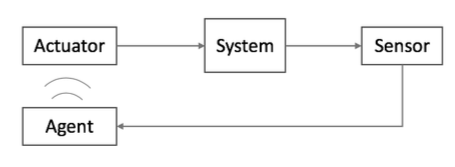
\includegraphics[width=10cm]{event.png}
 	\caption{control system} \label{image}
\end{figure}
Here, the system to be controlled is a continuous-time system is given by
\begin{equation}
	\dot{s} = h(s(t),u(t)) + \dot{w}\label{continuous_system}.
\end{equation}
where $u$ and $\dot{w}$ denote control input and process noise.\par
In this paper, we call the observation of the state variable $s$ and the sending of the input signal to the actuator as ``interaction". In the self-triggered control, the agent makes interaction not continuously, but after a communication interval $\tau$ determined by the agent itself. In order to express it mathematically, we assume that the agent's control law $\pi$ is a vector-valued function consisting of two elements, where the first element represents the input $u$ sent to the actuator, and the second element represents the interval $\tau$. Let $t_i$ be the time of the $i$-th communication, and $u_i$ be the input sent at $t_i$. The actuator continues to input $u_i$ until the next communication time. That is, the control input $u(t)$ at time $t$ is 
\begin{equation}
	u(t) = u_i, \forall t \in [t_i, t_{i+1}).
\end{equation} 
This control method is called Zero Order Hold (ZOH).

\subsection{Previous Research}
Several previous researches in self-triggered control make one step optimization of the next triggering time on each interaction. For example, \cite{STC} proposed the self-triggered control strategy for discrete time linear system
\begin{equation*}
	s_{i+1} = As_i + Bu_i + Dw_i
\end{equation*}
where $w_i$ is a white noise which satisfies $\expect[w_i] = 0$ and $\expect[w_iw_i^{\top}]=I$, where $I$  is a identity matrix.
They attempted to design a self-triggered control law that reduces the control cost from given initial state $s_0$
\begin{equation*}
	J = \sum_{i = 0}^{\infty}\expect[\alpha^i(s_i^{\top}Es_i+u_i^{\top}Fu_i)|s_0]
\end{equation*}
while keeping the interaction interval as long as possible. $E$ and $F$ are hyper parameter matrices. For the purpose, they proposed a method to adopt the maximum interval steps $\eta$ such that 
there exists an input $u$ satisfying
\begin{equation*}
	\expect[\sum_{j=0}^{\eta-1}\alpha^{j}(s_j^{\top}Es_j+u^{\top}Fu)+\alpha^{\eta}V(s^{\prime})|s_0=s] \leq V(s)
\end{equation*}
where
\begin{equation*}
	V(s) = \beta_1s^{\top}Ps + \beta_2\frac{\alpha}{1-\alpha}\textrm{tr}(PDD^{\top})
\end{equation*}
is not empty. Here, $\alpha, \beta_1, \beta_2$ is a hyper parameters, and $P$ is a unique positive definite solution of discrete time algebraic riccati equation 
\begin{equation*}
	P = A^\mathsf{T}PA-A^\mathsf{T}PB\left(F+B^\mathsf{T}PB\right)^{-1}B^\mathsf{T}PA+E.
\end{equation*}
In other words, they designed a self-triggered control law which has a cost function $V(s_0)$ as a performance guarantee. \par
Also, \cite{ECBF} proposed the self-triggered control strategy for continuous time control affine system 
\begin{equation*}
	\dot{s} = f(s(t)) + g(s(t))u(t).
\end{equation*}
The control input $u$ is defined as a solution of Quadratic Program, such as
\begin{align*}
	\min_{u}~~&u^{\top}u \\
	\textrm{s.t.}~~&\mathcal{L}_fV(s)+\mathcal{L}_gV(s)u+\varepsilon V(s)\leq 0
\end{align*}
where $\mathcal{L}_f, \mathcal{L}_g$ denote Lie derivatives, $\varepsilon$ is a hyperparameter and $V$ is a Lyapunov function. Then, select the maximum interval time $\tau$ where the Lyapunov function $V$ decreases at the next step. However, these approaches do not guarantee the optimality for the long-term control cost. \par
In this research, we formulate an optimal self-triggered control problem in which communication is explicitly included in the long-term control cost. This makes it possible to consider the problem of finding a control policy with a long-term cost, instead of a one-step optimization.

\subsection{Optimal Self-Triggered Control}
\label{sec:formulation}
In self-triggered control, the agent needs to decide the input signal $u$ and the interval $\tau$ at each step. Thus, the action $a$ in reinforcement learning corresponds to $\begin{bmatrix}u & \tau \end{bmatrix}^{\top}$. (In this paper, we equate $a$ with the tuple $(u,\tau)$.) \par
Now, in this research, the control law is given as a state feedback. Therefore, the policy function is given as follows.
\begin{equation}
	\pi(s) = \begin{bmatrix}u(s) & \tau(s)\end{bmatrix}^{\top}
\end{equation}
In order to make the state $s$ converge to the origin as quickly as possible with the minimum input energy while reducing the frequency of communication, the agent aims to find a policy $\pi^{*}$ that minimizes the following expected discounted cost 
\begin{equation}
	J(\pi)=\expect_{s\sim d_0}[V^{\pi}(s)] \label{evaluation}
\end{equation}
where
\begin{equation}
	V^{\pi}(s) = \expect_{w}\left[\int_{0}^{\infty} e^{-\alpha t}\{s(t)^{\top}Es(t)+u(t)^{\top}Fu(t)\}\textrm{d}t + \beta\sum_{t\in T_c}e^{-\alpha t}|s(0)=s\right]\label{such_that}
\end{equation}
and $T_c$ is the history of the communication time when controlled by the policy $\pi$.  If we separate the definite integral for each interval, we have 
\begin{align}
	V^{\pi}(s) &= \expect_{w}\left[\int_{0}^{\infty} e^{-\alpha t}\{s(t)^{\top}Es(t)+u(t)^{\top}Fu(t)\}\textrm{d}t + \beta\sum_{t\in T_c}e^{-\alpha t}|s(0)=s\right] \nonumber \\
			 &= \expect_w\left[\sum_{i=0}^{\infty} e^{-\alpha t_i} \left(\int_{0}^{\tau_i}e^{-\alpha t}\expect_{w}[s(t)^{\top}Es(t)+u_i^{\top}Fu_i|s(0)=s_i]\textrm{d}t + \beta\right)|s(0)=s\right] \nonumber \\
			 &= \expect_w\left[\sum_{i=0}^{\infty} e^{-\alpha t_i} r(s_i, \pi(s_i))|s(0)=s\right] \label{self_acc_reward}.
\end{align}
Here, $t_i$ is the time of the $i$-th communication and $s_i$ is the state at that time. Also, let $[u_i, \tau_i]=\pi(s_i)$, and the reward function $r(s, u, \tau)$ of each step as
\begin{equation}
	r(s, u, \tau) = \int_{0}^{\tau}e^{-\alpha t}\expect_{w}[s(t)^{\top}Es(t)+u^{\top}Fu|s(0)=s]\textrm{d}t + \beta.
\end{equation}
Therefore, $V^{\pi}(s)$ satisfies the following Bellman equation. \par
\begin{equation}
	V^{\pi}(s) = r(s,\pi(s)) + e^{-\alpha\tau(s)}\expect_{s^{\prime}}[V^{\pi}(s^{\prime}(s,\pi(s)))] \label{bellman}
\end{equation}
In addition, the action value function $Q^{\pi}$ is the discounted accumulation cost when the agent freely chooses an action in the first step and follows the policy $\pi$ from the next step, which satisfies the following Bellman equation.
\begin{equation}
	Q^{\pi}(s,u,\tau) = r(s,u,\tau) + e^{-\alpha\tau}\expect_{s^{\prime}}[Q^{\pi}(s^{\prime}(s,u,\tau), \pi(s^{\prime}(s,u,\tau)))] \label{Q_bellman}
\end{equation}

\section{Reinforcement Learning for Self-Triggered Control}
In this section, we consider an application of reinforcement learning to find the optimal self-trigger policy $\pi^{*}$. Simply thinking, we can formulate it as a reinforcement learning problem by taking the interaction as one step. Furthermore, DDPG may also be applied by approximating the $Q$ function, which satisfies the equation \eqref{Q_bellman} using a critic network, to obtain the policy gradient. In this section, we discuss the validity of this approach.

\subsection{Deterministic Policy Gradient for Self-Triggered Control}
Since the discount factor in Equation \eqref{self_acc_reward} depends on $\tau$ at each step, it differs from the general reinforcement learning problem. In this subsection, we discuss how the DPG is affected by this difference. \par
Actually, due to the property of $Q$ functions such as \eqref{Q_bellman}, DPG cannot be computed as in \eqref{true_pg}. Since 
\begin{align}
	\nabla_{\theta}V^{\pi_{\theta}}(s) &= \nabla_{\theta}Q^{\pi_{\theta}}(s, \pi_{\theta}(s)) \nonumber \\
	&= \nabla_{\theta}[r(s, \pi_{\theta}(s)) + e^{-\alpha\tau_{\theta}(s)}\expect_{s^{\prime}}[V^{\pi_{\theta}}(s^{\prime})] \nonumber \\
	&= \nabla_{\theta}\pi_{\theta}(s)\nabla_ar(s,a)|_{a=\pi_{\theta}(s)} \nonumber \\
	&\hspace{1ex}+e^{-\alpha\tau_{\theta}(s)}\int_{S}\{\nabla_{\theta}\pi_{\theta}(s)\nabla_aPr(s\to s^{\prime},1,a)|_{a=\pi(s)}V^{\pi_{\theta}}(s^{\prime})\nonumber\\
	&\hspace{15ex}+Pr(s\to s^{\prime}, 1, \pi_{\theta})\nabla_{\theta}V^{\pi_{\theta}}(s^{\prime})\}ds^{\prime}\nonumber \\
	&\hspace{1ex}+\int_{S}\nabla_{\theta}e^{-\alpha\tau_{\theta}(s)}Pr(s\to s^{\prime}, 1, \pi_{\theta})V^{\pi_{\theta}}(s^{\prime})ds^{\prime},
\end{align}
we have
\begin{align}
	&\nabla_{\theta}V^{\pi_{\theta}}(s) \nonumber \\
	&= \sum_{i=0}^{\infty}\int_{S}\cdots\int_{S}Pr(s_0\to s_1,1,\pi_{\theta})\cdots Pr(s_{i-1}\to s_i,1,\pi_{\theta})\nonumber\\
	&\hspace{10ex}e^{-\alpha t_i}\nabla_{\theta}\pi_{\theta}(s_i)\nabla_aQ^{\pi_{\theta}}(s_i,a)|_{a=\pi_{\theta}(s_i)}ds_ids_{i-1}\ldots ds_1\nonumber\\
	&\hspace{1ex}+\sum_{i=1}^{\infty}\int_{S}\cdots\int_{S}Pr(s_0\to s_1,1,\pi_{\theta})\cdots Pr(s_{i-1}\to s_i,1,\pi_{\theta})\nonumber\\
	&\hspace{10ex}e^{-\alpha t_{i-1}}\nabla_{\theta}e^{-\alpha\tau_{\theta}(s_{i-1})}V^{\pi_{\theta}}(s_{i})ds_ids_{i-1}\ldots ds_1\nonumber\\
	&= \sum_{i=0}^{\infty}\int_{S}\cdots\int_{S}Pr(s_0\to s_1,1,\pi_{\theta})\cdots Pr(s_{i-1}\to s_i,1,\pi_{\theta})\nonumber\\
	&\hspace{10ex}e^{-\alpha t_i}\nabla_{\theta}\pi_{\theta}(s_i)\nabla_aQ^{\pi_{\theta}}(s_i,a)|_{a=\pi_{\theta}(s_i)}ds_ids_{i-1}\ldots ds_1\nonumber\\
	&\hspace{1ex}+\sum_{i=0}^{\infty}\int_{S}\cdots\int_{S}Pr(s_0\to s_1,1,\pi_{\theta})\cdots Pr(s_{i}\to s_{i+1},1,\pi_{\theta})\nonumber\\
	&\hspace{10ex}e^{-\alpha t_{i}}\nabla_{\theta}e^{-\alpha\tau_{\theta}(s_{i})}V^{\pi_{\theta}}(s_{i+1})ds_{i+1}ds_{i}\ldots ds_1,
\end{align}
where 
\begin{equation}
	t_i = \begin{cases}
    		0 & (i=0) \\
    		\sum_{k=0}^{i-1}\tau_{\theta}(s_{k-1}) & (otherwise)
  		\end{cases}.
\end{equation}\par
Now, since $J(\pi_{\theta}) = \expect_{s_0\sim d_0}[V^{\pi_{\theta}}(s_0)]$, we have deterministic policy gradient theorem for self-triggered control.

\begin{th.}[Deterministic Policy Gradient Theorem for Self-Triggered Control]
\label{main_theorem}
The gradient for evaluation function \eqref{evaluation}, \eqref{such_that} is given by
\begin{align}
	&\nabla_{\theta}J(\pi_{\theta})\nonumber \\
	&= \expect_{s_0\sim d_0}[\nabla_{\theta}V^{\pi_{\theta}}(s_0)]\nonumber\\
	&= \sum_{i=0}^{\infty}\int_{S}\cdots\int_{S}d_0(s_0)Pr(s_0\to s_1,1,\pi_{\theta})\cdots Pr(s_{i}\to s_{i+1},1,\pi_{\theta})\nonumber\\
	&\hspace{5ex}e^{-\alpha t_i}\{\nabla_{\theta}\pi_{\theta}(s_i)\nabla_aQ^{\pi_{\theta}}(s_i,a)|_{a=\pi_{\theta}(s_i)} + \nabla_{\theta}e^{-\alpha\tau_{\theta}(s_{i})}V^{\pi_{\theta}}(s_{i+1})\}ds_{i+1}ds_{i}\ldots ds_0. \label{PG_for_STC}
\end{align}
\end{th.}

\subsection{Value Function for Self-Triggered Control}
In DPG for reinforcement learning problems with a fixed discount factor, it is sufficient that the gradient $\nabla_aQ(s,a|\omega)|_{a=\pi(s)}$ can correctly approximate $\nabla_aQ^{\pi(s)}(s,a)|_{a=\pi(s)}$. However from equation \eqref{PG_for_STC}, in the case of reinforcement learning for self-triggered control considered in this paper, the value of $V^{\pi}(s)$ itself must also be correctly approximated. Therefore, we need to pay attention to the TD learning of critic.\par
Since the value function $V^{\pi}(s)$ satisfies 
\begin{equation}
	V^{\pi}(s) = Q^{\pi}(s,\pi(s)),
\end{equation}
we consider a TD learning algorithm that enables the critic to correctly approximate $\nabla_aQ^{\pi}(s,a)|_{a=\pi(s)}$ and $Q^{\pi}(s,\pi(s))$. First, we discuss how to create a dataset $D$ for training. If the distribution of the state $s$ in the training dataset is biased, the accuracy of the function approximation for the state $s$ which is not in the distribution will be low. Also, for the calculation of $\nabla_aQ(s,a|\omega)|_{a=\pi(s)}$, it is necessary that the action $a$ is distributed around the trajectory of $\pi(s)$. Then, on the state space $S$, we sample $M$ states $s$ with equal probability, and for each state $s$ we choose 
\begin{equation}
	[u, \tau] = \pi(s) + e
\end{equation}
and input $u$ for the time $\tau$. (where $e$ is an exploration noise). The resulting reward $r$ and the next state $s^{\prime}$ are observed, and the data tuple $(s,u,\tau,r,s^{\prime})$ is stored in the dataset $D$. Note that, considering the stochasticity of action selection and system noise, we collect data from each state $s$ for $R$ times.\par
Concerning the regression criterion, $Q^{\pi}(s,u, \tau)$ make the TD error
\begin{equation}
	TD = Q(s,u,\tau|\omega) - \{r(s,u,\tau) + e^{-\alpha\tau}\expect_{s^{\prime}}[Q(s^{\prime}(s,u,\tau), \pi(s^{\prime}(s,u,\tau))|\omega)]\}
\end{equation} 
to be zero. Thus, the critic is trained by repeatedly creating a mini-batch $E$ by sampling $m$ data from the dataset $D$, and updating the critic parameter $\omega$ toward decreasing the MSE of the TD error for the mini-batch $E$, using the gradient
\begin{equation}
	g = \pdif{}{\omega}\left[\frac{1}{m}\sum_{(s,u,\tau,r,s^{\prime})\in E}\left(Q(s,u,\tau|\omega) - \{r + e^{-\alpha\tau}Q(s^{\prime}, \pi(s^{\prime})|\omega)\}\right)^2\right].
\end{equation}
Algorithm \ref{alg1} shows the learning algorithm for the critic described in this section.
\begin{algorithm}                      
\caption{TD Learning for Critic Network}         
\label{alg1}                          
\begin{algorithmic}                  
    \STATE Sample $M$ states $s$ with equal probability from state space $S$.
    \FOR {$r = 0$ to $R$}
    	\STATE For all sampled $s$, choose $[u, \tau]=\pi(s) + e$.
	\STATE Execute action $u$ for time $\tau$ to the environment.
	\STATE Receive $r$ and observe next state $s^{\prime}$.
	\STATE Store $(s, u, \tau, r, s^{\prime})$ to data set $D$.
    \ENDFOR
    \FOR {$\textrm{epoch} = 0$ to $N$}
    	\STATE Select $m$ data pairs $(s, u, \tau, r, s^{\prime})$ from $D$ and make a mini-batch $E$.
	\STATE Calculate gradient $g = \pdif{}{\omega} \frac{1}{m}\sum_{E}\left(Q(s,u,\tau|\omega) - \{r + e^{-\alpha\tau}Q(s^{\prime}, \pi(s^{\prime})|\omega)\}\right)^2$.
	\STATE Update $\omega$ with gradient $g$.
    \ENDFOR
    \end{algorithmic}
\end{algorithm}\par
At the end part of this section, we check the approximation accuracy of the critic learned by using Algorithm \ref{alg1}. Unfortunately, it is difficult to compute $\nabla_aQ^{\pi}(s,a)|_{a=\pi(s)}$ for the true $Q$ function, so we only check the approximation accuracy of $Q(s,\pi(s)|\omega)$ for the value function $V^{\pi}(s)$. Both $V^{\pi}(s)$ and $Q(s, \pi(s)|\omega)$ are functions of state $s$. The state $s$ is assumed to be two-dimensional, and the comparison between them is shown in Figure \ref{Q_approximation}. 
\begin{figure}[H]
	\centering
 	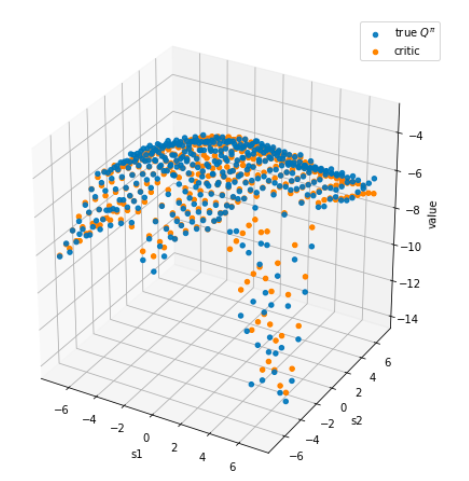
\includegraphics[width=10cm]{Q_approximation.png}
 	\caption{Approximation of $Q^{\pi}(s,\pi(s))$} \label{Q_approximation}
\end{figure}
In Figure \ref{Q_approximation}, the blue points indicate the true $V^{\pi}$ and the orange points indicate the critics. The true $V^{\pi}$ is obtained by simulation. 
In this case, the average of the relative error
\begin{equation}
	\frac{|V^{\pi}(s)-Q(s, \pi(s)|\omega)|}{|V^{\pi}(s)|}
\end{equation}
at points shown in Figure \ref{Q_approximation} is 0.03. Thus, we can consider that the critic learned by Algorithm \ref{alg1} is a good approximation of $V^{\pi}$. The dependency of computation complexity for dimension of state $s$ should be studied in the future.

\subsection{Naive Implementation}
We start by considering an naive implementation for computing the exact policy gradient \eqref{PG_for_STC} without considering the computational complexity. Assume that the critic is learned with Alrogithm \ref{alg1}. Equation \eqref{PG_for_STC} is the expectation of
\begin{equation}
	\sum_{i=0}^{\infty} e^{-\alpha t_i}\{\nabla_{\theta}\pi_{\theta}(s_i)\nabla_{a}Q(s,a|\omega)|_{a=\pi_{\theta}(s_i)} + \nabla_{\theta}e^{-\alpha\tau_{\theta}(s_{i})}Q(s_{i+1},\pi_{\theta}(s_{i+1})|\omega)\} \label{path_gradient}
\end{equation}
with respect to the stochasticity of the initial state distribution and the system noise. We consider the method of approximate calculations of \eqref{PG_for_STC} on the computer. For an initial state distribution $d_0$, we generate $M$ initial states $s_0$, then $P$ times controls are performed from each $s_0$ for time $T$, and
\begin{equation}
	\sum_{i\in T_i} e^{-\alpha t_i}\{\nabla_{\theta}\pi_{\theta}(s_i)\nabla_{a}Q(s,a|\omega)|_{a=\pi_{\theta}(s_i)} + \nabla_{\theta}e^{-\alpha\tau_{\theta}(s_{i})}Q(s_{i+1},\pi_{\theta}(s_{i+1})|\omega)\} \label{good_approximation_of_STCDPG}
\end{equation}
is calculated using all data pairs $(s_i,s_{i+1}, t_i)$ experienced on each control. Here, let $T_i$ be the set $\{i~|~t_i \leq T\}$. If we take $P, T$ and $M$ to be infinitely large, and if $Q(s,a|\omega)$ is a good approximation of $Q^{\pi_{\theta}}(s,a)$, The average of the computed results of \eqref{good_approximation_of_STCDPG} for all control paths is considered to be a good approximation of \eqref{PG_for_STC}. In algorighm \ref{alg2}, the reinforcement learning method with ideal calculation of policy gradient at each step. 
\begin{algorithm}                      
\caption{Naive Implementation of Self-Triggered Control RL}         
\label{alg2}                          
\begin{algorithmic}                  
    \STATE Initialize actor $\pi_{\theta}(s)$ and critic $Q(s,u,\tau|\omega)$.
    \STATE Learn the critic $Q(s,u,\tau|\omega)$ with algorithm \ref{alg1}.
    \FOR {$epoch=0$ to $N$}
        \FOR {$m = 0$ to $M$}
            \STATE Initialize $s_0\sim d_0$.
        \FOR {$\textrm{episode} = 0$ to $P$}
            \STATE Initialize episode memory $H$.
                \WHILE {$t \leq T$}
                \STATE Select $[u, \tau] = \pi_{\theta}(s)$.
                \STATE Execute action $u$ for time $\tau$ to the environment.
                \STATE Receive $r$ and observe next state $s^{\prime}$.
                \STATE Store tuple $(s, s^{\prime}, t)$ to the episode memory $H$.
            \ENDWHILE
            \STATE Calculate \eqref{good_approximation_of_STCDPG} with episode memory $H$.
        \ENDFOR
        \STATE Take the average of \eqref{good_approximation_of_STCDPG} over $P$ paths, and let it be $V^{\pi_{\theta}}(s_0)$.
        \ENDFOR
    \ENDFOR
    \STATE Take the average of $V^{\pi_{\theta}}(s_0)$ over the generated $s_0$ and let it be policy gradient $g$.
    \STATE Update the actor with approximated policy gradient $g$.
   \end{algorithmic}
\end{algorithm}

\subsection{Practical Implementation}
As mentioned before, the above algorithm does not take into account the problem of computational complexity. We consider an efficient method to approximate the policy gradient inspiered by DDPG. The most important point is the state distribution of the mini-batch which takes the sample mean to approximate equation \eqref{PG_for_STC}. \par
During the training, the agent decide
\begin{equation}
	[u_i, \tau_i] = \pi_{\theta}(s_i) + e_i
\end{equation}
and input $u_i$ for time $\tau$ on each steps ($e_i$ is an exploration noise). We observe the reward $r_i$ and the next state $s_{i+1}$, and store the data tuple $(s_i, u_i, \tau_i, r_i, s_{i+1}, t_i)$ in the replay buffer. It differs from DDPG in that the time $t_i$ from the start of control is stored in the replay buffer. In order to bring the diversity of data in the replay buffer, we assume that after every fixed time duration $T$, the initial state $s_0$ is generated and the control is replayed again. Assuming that the actor is updated only gradually, the replay buffer stores the experience gained by policies similar to the current policy. Thus, if we create a mini-batch $E$ by sampling the experience with probability $e^{-\alpha t_i}$, we can expect that the sample mean
\begin{equation}
	\frac{1}{M}\sum_{(s, s^{\prime})\in E}\{\nabla_{\theta}\pi_{\theta}(s)\nabla_{a}Q(s,a|\omega)|_{a=\pi_{\theta}(s)}+\nabla_{\theta}e^{-\alpha\tau_{\theta}(s)}Q(s, \pi_{\theta}(s)|\omega)\} \label{app_pg_stc}
\end{equation}
for the mini-batch $E$ will approximate \eqref{PG_for_STC} well. This is because the distribution of the mini-batch $E$ is discounted for $e^{-\alpha t}$. \par
On the other hand, the critic is updated by reducing the MSE of TD error for mini-batch $E$. However, it is known that if the the target value 
\begin{equation}
	r + e^{-\alpha\tau}Q(s^{\prime}, \pi_{\theta}(s^{\prime})|\omega)
\end{equation}
is calculated with the actor $\pi_{\theta}(s)$ and the critic $Q(s,a|\omega)$, the learning proved to be unstable in many environments \cite{ETC},\cite{DDPG}. So, as in DQN and DDPG, we use target networks to stabilize the training. Target networks $\pi_{\theta^{\prime}}(s), Q(s,a|\omega^{\prime})$ are created as copies of $\pi_{\theta}(s), Q(s,a|\omega)$, and used only for the calculation of the target value. That is, the critic is updated using the gradient
\begin{equation}
	g = \pdif{}{\omega}\left[\frac{1}{m}\sum_{(s,u,\tau,r,s^{\prime})\in E}\left(Q(s,u,\tau|\omega) - \{r + e^{-\alpha\tau}Q(s^{\prime}, \pi_{\theta^{\prime}}(s^{\prime})|\omega^{\prime})\}\right)^2\right].
\end{equation}
After the update of $\theta$ and $\omega$, the parameters of target networks are updated as
\begin{equation}
  \begin{split}
  	\theta^{\prime} &\gets (1-\xi)\theta^{\prime} + \xi\theta \\
	\omega^{\prime} &\gets (1-\xi)\omega^{\prime} + \xi\omega \label{target}
  \end{split}
\end{equation}
with a hyper parameter $\xi\ll1$.\par
Algorithm \ref{alg3} shows the efficient algorithm utilizing these idea.
\begin{algorithm}                      
\caption{Practical Implementation of Self-Triggered Control RL}         
\label{alg3}                          
\begin{algorithmic}                  
    \STATE Initialize the actor $\pi_{\theta}(s)$ and the critic $Q(s,u,\tau|\omega)$.
    \STATE Make target networks $\pi_{\theta^{\prime}}(s)$ and $Q(s,u,\tau|\omega^{\prime})$ by cloning the actor and the critic respectively.
    \FOR {$\textrm{episode} = 0$ to $M$}
    	\STATE Initialize $s_0\in d_0$.
    	\STATE Set $i = 0, t_i = 0$.
    	\WHILE {$t_i \leq T$}
    		\STATE Select $[u_i, \tau_i] = \pi_{\theta}(s_i) + e_i$.
		\STATE Execute action $u_i$ for time $\tau_i$ to the environment.
		\STATE Receive $r_i$ and observe $s_{i+1}$.
		\STATE Store $(s_i, u_i, \tau_i, r_i, s_{i+1}, t_i)$ to the replay buffer.
		\STATE Make mini-batch $E$ considering probability $e^{-\alpha t_i}$.
		\STATE Update the critic $\omega$ to decrease 
			\[L = \sum_{(s,u,\tau)\in E}Q(s,u,\tau|\omega) - \{r(s,u,\tau) + e^{-\alpha\tau}Q(s^{\prime}, \pi_{\theta^{\prime}}(s^{\prime})|\omega^{\prime})\}.\]
		\STATE Calculate approximated policy gradient using \eqref{app_pg_stc}.
		\STATE Update the actor with approximated policy gradient.
		\STATE Update target networks as \eqref{target}.
    	\ENDWHILE
    \ENDFOR
\end{algorithmic}
\end{algorithm}
We refer to Algorithm \ref{alg3} as the proposed method.

\section{Numerical Experiment}
In this section, we study the effectiveness of the reinforcement learning approach to the optimal self-triggered control problem. We conduct numerical experiments and review the results for the cases of linear and nonlinear control systems, respectively. In both cases, the communication interval is allowed to be 
\begin{equation}
	0.01 \leq \tau \leq 10.0
\end{equation}

\subsection{Evaluation Criteria}
In this section, we use the valuation function $J(\pi)$ as a criterion to evaluate the policy $\pi$. $J(\pi)$ is the expectation of the value function $V^{\pi}(s)$ with respect to the initial state distribution $s_0$. In this paper, we assume that the initial state distribution $d_0$ is a uniform distribution on the initial state space $S$ in both linear and nonlinear cases. Then, the space $S$ is discretized into a grid, and the value function $V^{\pi}(s)$ for each state $s$ on the grid is calculated by simulation and averaged to approximate the valuation function $J(\pi)$. In order to take into account the effect of system noise, $V^{\pi}(s)$ is the average of the long-time costs of several simulations for each state $s$.\par

\subsection{Linear System}
First, we adopt reinforcement learning to self-triggered control for linear system. The system to be controlled is
\begin{equation}
	\dot{s} = As + Bu + D\dot{w}= \begin{bmatrix}-1& 4 \\ 2 & -3\end{bmatrix}s + \begin{bmatrix}2 \\ 4\end{bmatrix}u + \begin{bmatrix}0.6 \\ 0.3\end{bmatrix}\dot{w}
\end{equation}
where $\dot{w}$ is wiener process noise. Here, the input signal $u$ is limited to $-10 \sim 10$. Let the initial state space be $S = \{s=[s_0, s_1]^{\top}\in \mathbb{R}^2| s_0\in[-7,7], s_1\in[-7,7]\}$. 
\if0
If an element of state $s$ exceed $[-7,7]$, it will be clipped to the edge of the range.
\fi

\subsubsection{Initial Policy}
For the comparison with the control performance with that of a naively designed model-based self-triggered control law, we use $\pi_{\textrm{MB}}(s)$ such that
\begin{equation}
	\pi_{\textrm{MB}}(s) = \argmin_{u,\tau} \left\{u^2 - \lambda\tau + {s^{\prime}_e}^{\top}Ps^{\prime} _e+ \textrm{Tr}(P\Sigma)\right\} \label{mb_objective}
\end{equation}
where $s^{\prime}_e=\expect_{w}[s^{\prime}(s,u,\tau)]$, $\Sigma=Var_w[s^{\prime}(s,u,\tau)]$ are  expectation and variance of next state respectively, and $P$ is a unique solution of continuous time algebraic riccati equation
\begin{equation}
	A^{\top}P + PA - PBF^{-1}B^{\top}P + E = \bm{0}
\end{equation}
where, $E$ and $F$ are hyper parameter matrix. The last two terms of objective function of \eqref{mb_objective} denotes the optimal cost of continuous control with the LQR controller from the following state $s^{\prime}_e$ for the system without noise. By incorporating this cost into the objective, we can find $u$ and $\tau$ such that the transition to the state which requires high control cost in the next step is avoided.\par 
In order to use $\pi_{\textrm{MB}}$ as an initial policy for reinforcement learning, we represent $\pi_{\textrm{MB}}$ as a neural network approximated by supervised learning of $\pi_{\textrm{MB}}(s)$ for $M$ randomly generated states $s$ in the state space $S$. The evaluation value of supervised $\pi_{\textrm{MB}}$ for several $\lambda$ are shown in Table \ref{ev}.
\begin{table}[htb]
  \begin{center}
    \begin{tabular}{|cc|} \hline
      $\lambda$ & $J(\pi)$ \\ \hline 
      0.01 & 22.14 \\
      0.1 & 80.02 \\ %?
      0.5 & 19.61 \\
      1.0 & 11.32 \\
      5.0 & 12.23 \\
      10 & 15.72 \\
      50 & 32.21 \\
      100 & 37.38 \\ \hline
    \end{tabular}
    \caption{Evaluation value for several $\lambda$}
    \label{ev}
  \end{center}
\end{table}
We refer to the best policy in Table \ref{ev} ($\lambda = 1.0$) as $\hat{\pi}_{\textrm{MB}}$ and use it as the initial policy for proposed method. Figure \ref{naiive} shows the control path with initial policy $\hat{\pi}_{\textrm{MB}}$ stating from $s_0 = [3., 3.]$.
\begin{figure}[H]
	\centering
 	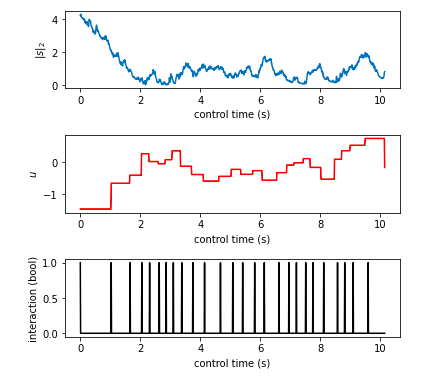
\includegraphics[width=8cm]{naiive.png}
 	\caption{A control path with learned policy $\hat{\pi}_{\textrm{MB}}$} \label{naiive}
\end{figure}
In Figure \ref{naiive}, the norm of state $s$, the control signal $u$ and the Boolean which denotes whether agent interact with environment at time $t$ are shown from top to bottom.

\subsubsection{Result of Proposed Method}
First, we consider the results of reinforcement learning using the proposed method 1 with $\hat{\pi}_{\textrm{MB}}$ as the initial policy. Figure \ref{proposed_1_linear} shows the path controlled by the policy $\pi_{\textrm{prop}}^L$ from the initial state $s_0=\begin{bmatrix}3 & 3\end{bmatrix}$.
\begin{figure}[t]
	\centering
 	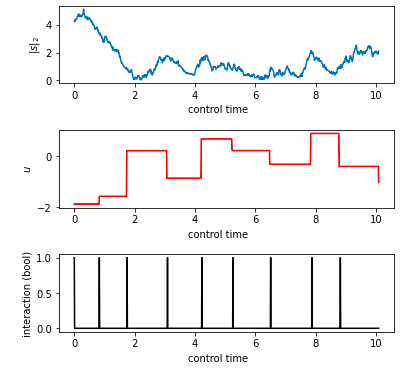
\includegraphics[width=8cm]{proposed_1_linear.png}
 	\caption{A control path with learned policy $\pi_{\textrm{prop}}^L$} \label{proposed_1_linear}
\end{figure}
\begin{figure}[H]
	\centering
 	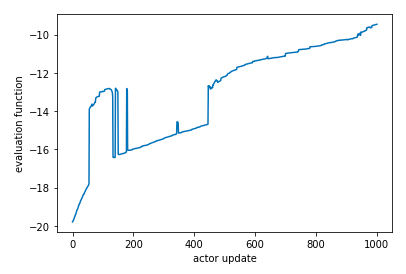
\includegraphics[width=10cm]{evaluation_log_linear.png}
 	\caption{Policy improvement on linear case} \label{evaluation_log_linear}
\end{figure}
The evaluation value of this policy $\pi_{\textrm{prop}}^L$ is
\begin{equation}
	J(\pi_{\textrm{prop}}^L) \simeq 6.82
\end{equation}
Thus, we can see the improvement of the policy from $\hat{\pi}_{\textrm{MB}}$.\par
The history of the value of the evaluation function $J( \pi_{\theta})$ as the policy parameter $\theta$ is updated is shown in Figure \ref{evaluation_log_linear}.
Figure \ref{evaluation_log_linear} shows an example of successful learning. However, since the calculation of the policy gradient depends on the approximation accuracy of the critic according to the equation \eqref{app_pg_stc}, we often observed a sharp deterioration of the policy using the proposed method. The learning accuracy of critic is a future work.

\subsection{Non-linear Case}
In this subsection, we investigate whether the self-triggered control law can be learned by reinforcement learning even when the control target is extended to non-linear systems, in particular  control affine systems. We consider an inverted pendulum, whose state-space representation is
\begin{equation}
	\odif{}{t}\begin{bmatrix}\phi \\ \dot{\phi}\end{bmatrix} = 
		\begin{bmatrix}\dot{\phi} \\ \frac{3g}{2l}\sin{\phi} + \frac{3}{ml^2}u \end{bmatrix} + \begin{bmatrix}1 \\ 1\end{bmatrix}\dot{w}\label{pendulum}.
\end{equation}
where $\dot{w}$ is wiener process noise. Therefore, for an inverted pendulum, the state variable $s$ is considered to be $\begin{pmatrix}\phi & \dot{\phi}\end{pmatrix}^{\top}$.
\par
As in the linear case, the input signal $u$ is limited to $-10 \sim 10$. And let the initial state space be $S = \{[\phi, \dot{\phi}]^{\top}\in \mathbb{R}^2| \phi\in[-\pi,\pi], \dot{\phi}\in[-2\pi,2\pi]\}$. 
\if0
If angle $\|\theta\| > \pi$, $\theta$ will be replaced by the equivalent angle which satisfies $\|\theta\| \leq \pi$. And if Angular velocity $\|\dot{\theta}\| > 2\pi$, $\|\dot{\theta}\|$ will be clipped to the edge of $[-2\pi,2\pi]\}$.
\fi

\subsubsection{Initial Policy}
The initial policy $\pi_{\textrm{init}}$ used in this case is
\begin{equation}
	\pi_{\textrm{init}}(s) = \begin{bmatrix}-Ks&0.2\end{bmatrix}
\end{equation}
where $K$ is a feedback gain calculated by Linear Quadratic Regulator for linearized system around $s = \bm{0}$. Figure \ref{sample_02} shows the control path with initial policy $\pi_{\textrm{init}}$ stating from $s_0 = [3., 3.]$.
\begin{figure}[h]
	\centering
 	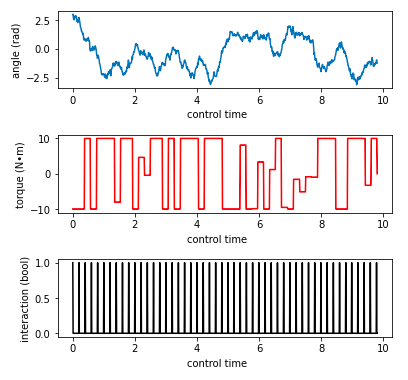
\includegraphics[width=8cm]{sample_02.png}
 	\caption{A control path with initial policy $\pi_{\textrm{init}}$} \label{sample_02}
\end{figure}\\
The evaluation value of $\pi_{\textrm{init}}$ is
\begin{equation}
	J(\pi_{\textrm{init}}) \simeq 62.49
\end{equation}
In Figure \ref{sample_02}, the angle of pendulum $\phi$ rad, the torque $u$ N$\cdot$m and the Boolean which denotes whether agent interact with environment at time $t$ are shown from top to bottom.

\subsubsection{Result of Proposed Method}
First, we show the results of reinforcement learning by the proposed method 1. Figure \ref{proposed_1_nl} shows the control path by the obtained policy $\pi_{\textrm{prop}}^N$ stating from $s_0 = [3., 3.]$.
\begin{figure}[t]
	\centering
 	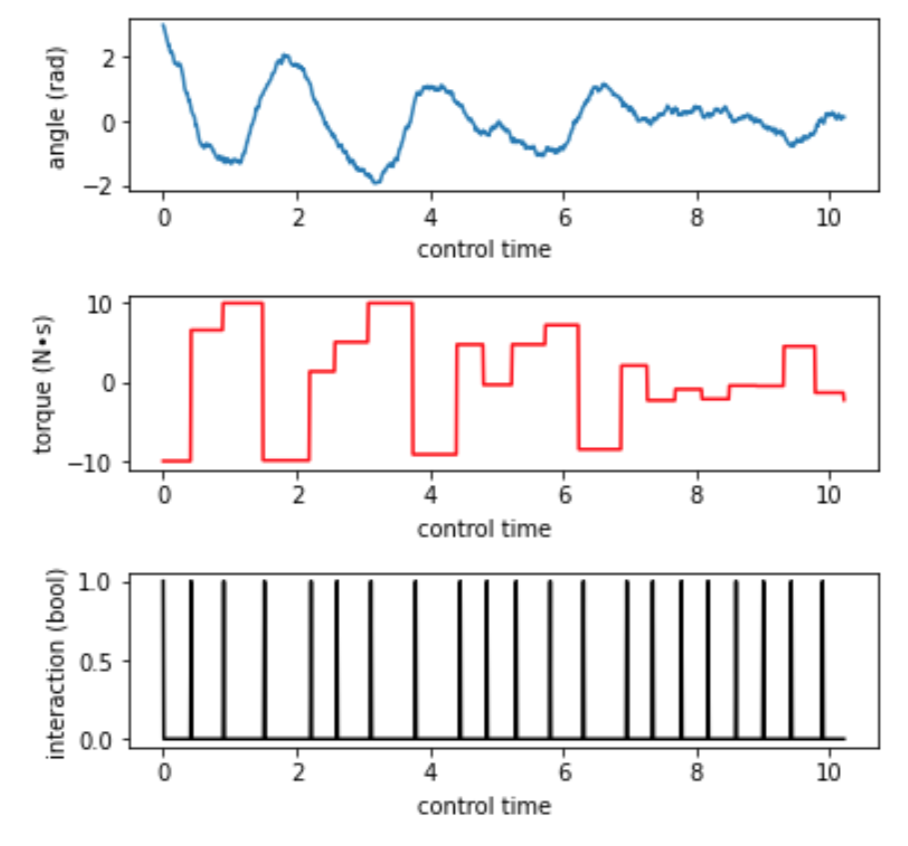
\includegraphics[width=8cm]{proposed_1_nl.png}
 	\caption{A control path with learned policy $\pi_{\textrm{prop}}^N$} \label{proposed_1_nl}
\end{figure}
The evaluation value of $\pi_{\textrm{prop}}^N$ is
\begin{equation}
	J(\pi_{\textrm{prop}}^N) \simeq 30.57
\end{equation}\\
Thus, we can confirm the improvement of the policy.\par
The change of the value of the evaluation function $J( \pi_{\theta})$ as the policy parameter $\theta$ is updated is shown in Figure \ref{evaluation_log_nl}.
\begin{figure}[H]
	\centering
 	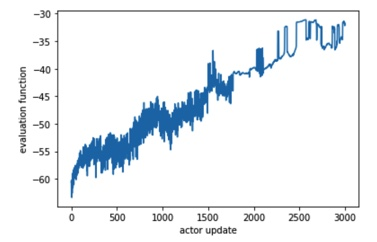
\includegraphics[width=10cm]{evaluation_log_nl.png}
 	\caption{Policy improvement on non-linear case} \label{evaluation_log_nl}
\end{figure}

\section{Conclusion}
In this paper, we formulated an optimal self-triggered control problem where the communication cost was explicitly included, which had not been considered in previous studies. Then, we considered a reinforcement learning approach to the problem.  \par
First, from the configuration of the evaluation function, we confirmed that the deterministic policy gradient theorem for general reinforcement learning was not directly applicable, and then we gave a policy gradient theorem that was compatible with the formulated optimal self-triggered control problem. \par
In this paper, we also proposed a reinforcement learning algorithm for approximate computation of the policy gradient. As a result of the implementation, for the linear system, we can improve the policy in the sense of the formulated evaluation function for the control law designedheuristically based on  the model. We also succeeded in improving the policy for self-triggered control of nonlinear systems, which was not solved in the previous study. \par
However, the computational complexity and the way of saving the empirical data are important issues to be solved in the future, because they greatly affect the results of the calculation of the policy gradient.

%%% Acknowledgments %%%%%%%%%%%%%%%%%%%%%%%%%%%%%%%%%%%%%%%%%%%%%%%%%%%%%%%%%%%%%
\acknowledgment
The author would like to express his sincere gratitude to Professor
Yoshito Ohta, Associate Professor Kenji Kashima and Assistant Professor Kentaro Ohki for their helpful advices. He would also like to thank his colleagues in the control systems theory field laboratory for discussing with him.

%%% References %%%%%%%%%%%%%%%%%%%%%%%%%%%%%%%%%%%%%%%%%%%%%%%%%%%%%%%%%%%%%%%%%%
\addcontentsline{toc}{section}{\refname} % Add to the table of contents.
                                         % Delete if you use chapter option.
\begin{thebibliography}{20}
\bibitem{ETC_intro}
W. P. M. H. Heemels, K. H. Johansson, and P. Tabuada. ``An introduction to event-triggered and self-triggered control.” \textit{In Proc. of the 51st IEEE International Conference on Decision and Control}, pp. 3270-3285, 2012.
\bibitem{ETC}
D. Baumann, J. J. Zhu, G. Martius, and S. Trimpe. ``Deep Reinforcement Learning for Event-Triggered Control.”  In \textit{Proc. of the 57th IEEE International Conference on Decision and Control}, pp. 943-950, 2018.
\bibitem{STC}
T. Gommans, D. Antunes, T. Donkers, P. Tabuada, and M. Heemels. ``Self-triggered linear quadratic control.” \textit{Automatica}, vol. 50, no. 4, pp. 1279-1287, 2014.
\bibitem{ECBF}
G. Yang, C. Belta, and R. Tron. ``Self-triggered Control for Safety Critical Systems Using Control Barrier Functions."  In \textit{Proc. of the American Control Conference},  pp. 4454-4459, 2019.
\bibitem{RL}
R. S. Sutton and A. G. Barto. \textit{Reinforcement Learning: An Introduction}, MIT Press, 1998.
\bibitem{Q}
C. J. Watkins, and P. Dayan. ``Q-learning." \textit{Machine Learning}, vol. 8, no. 3-4, pp. 279-292, 1992.
\bibitem{DQN}
V. Minh, et al. ``Human-level control through deep reinforcement learning." \textit{Nature 518}, pp.529-533, 2015.
\bibitem{DPG}
D. Silver, G. Lever, N. Heess, T. Degris, D. Wierstra and M. Riedmiller. ``Deterministic Policy Gradient Algorithms." In \textit{Proc. of the 31st International Conference on Machine Learning}, pp. 387-395, 2014.
\bibitem{DDPG}
T. P. Lillicrap, J. J. Hunt, A. Pritzel, N.Heess, T. Erez, Y. Tassa, D. Silver, and D. Wierstra. ``Continuous control with deep reinforcement learning." In \textit{Proc. of the 4th International Conference on Learning Representations}, 2016; arXiv: 1509.02971 v6.
\bibitem{survey}
I. Grondman, L. Busoniu, G. A. Lopes, and R. Babuska. ``A Survey of Actor-Critic Reinforcement Learning: Standard and Natural Policy Gradient." \textit{IEEE Transactions on Systems, Man, and Cybernetics, Part C (Applications and Reviews)}, vol. 42, no. 6, pp. 1291-1307, 2012.
\bibitem{off-PAC}
T. Degris, M. White and R. S. Sutton. ``Off-Policy Actor-Critic." In \textit{Proc. of the 29th International Conference on Machine Learning}, pp.179-186, 2012.
\bibitem{approximation}
R. S. Sutton, D. McAllester, S. Singh, and Y. Mansour. ``Policy gradient methods for reinforcement learning with function approximation." In \textit{Advances in Neural Information Processing Systems}, pp. 1057-1063, 2000.
\bibitem{Adam}
D. P. Kingma and J. Ba. ``Adam: A Method for Stochastic Optimization." In \textit{Proc. of the 3rd International Conference on Learning Representations}, 2015; arXiv: 1412.6980 v9.
\bibitem{rein}
T. Morimura. \textit{Reinforcement Learning}, Koudansha, 2019 (In Japanese).
\bibitem{stochastic}
A. Ohsumi. \textit{Introduction to Stochastic Systems}, Asakura Publishing, 2002 (In Japanese).

\end{thebibliography}
%%% If you want to use BibTeX, delete the above and insert code here.
%% \bibliographystyle{...}
%% \bibliography{...}

%%% Appendix %%%%%%%%%%%%%%%%%%%%%%%%%%%%%%%%%%%%%%%%%%%%%%%%%%%%%%%%%%%%%%%%%%%%
%%% If you don't need appendices, delete the below.
\appendix

\section{Appendix}
\subsection{Model Settings}
We use the actor-critic method. The actor and the critic are expressed as neural networks respectively. In numerical evaluation in Section 5, specific networks of the architecture in Figure \ref{NN} are implemented. The architecture of 2 networks is in Figure \ref{NN}.
The activation function ``original" shown in Figure \ref{NN} is defined as $9.99 \times \textrm{sigmoid} + 0.01$ to meet upper and lower limits of interval described in section 5.2 and 5.3.
\begin{figure}[h]
	\centering
 	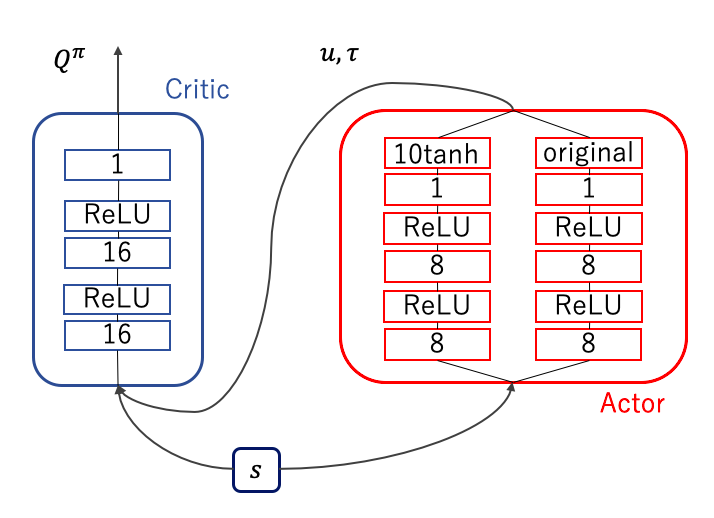
\includegraphics[width=10cm]{model.png}
 	\caption{Agent Model} \label{NN}
\end{figure}

%%% End of body %%%%%%%%%%%%%%%%%%%%%%%%%%%%%%%%%%%%%%%%%%%%%%%%%%%%%%%%%%%%%%%%%
\fi
\ifoutputcover
\cleardoublepage
%%% Covers and abstract for submission %%%%%%%%%%%%%%%%%%%%%%%%%%%%%%%%%%%%%%%%%%
\makecover                      % Cover
\makespine[\numberofspines]     % Spine
\fi
\ifoutputabstractforsubmission
\makeabstractforsubmission      % Abstract for submission
\fi
\end{document}
